\documentclass[11pt]{article}
\usepackage[margin=1in]{geometry}
\usepackage{amsmath,amssymb}
\usepackage{graphicx}
\usepackage{booktabs}
\usepackage[colorlinks=true,linkcolor=blue,citecolor=blue,urlcolor=blue]{hyperref}

\title{A correlation-scaled independence approximation for fork-join queues with general service times:
a preregistered evaluation}
\author{Singularity}
\date{\today}

\begin{document}
\maketitle

\begin{abstract}
The mean response time of a fork-join queue with $K\ge3$ parallel FCFS servers has no known closed form. The
approximations in common use either assume exponential service (Nelson--Tantawi, Varma--Makowski) or rely only on
the first two moments of the single-queue response time (the extreme-value approximation). We propose
\[
T_K\approx R+\phi\,(R^{\max}_K-R),\qquad \phi=(1-r)^{\rho h},\qquad r=\frac{1}{1+c^2},
\]
where $R$ is the exact M/G/1 mean response time and $R^{\max}_K$ is the classical upper bound: the exact mean of the
maximum of $K$ independent M/G/1 response times, obtained from the Pollaczek--Khinchine transform by FFT. The factor
$\phi$ accounts for the positive correlation that arrivals induce among the servers. Here $c^2$ is the squared
coefficient of variation of service, and $h$ is a five-parameter function of $\rho$, $r$ and $\sqrt{\ln K}$.

The functional form was found in an exploration phase in which a Kolmogorov--Arnold network suggested the
$\sqrt{\ln K}$ dependence. It was then tested once, in a preregistered confirmation on simulated data that was not
used to choose or fit it.
\begin{itemize}
\item \textbf{Exponential service}, $K\le128$: the maximum error is $1.03\%$, against $3.23\%$ for Nelson--Tantawi and
$10.98\%$ for Varma--Makowski.
\item \textbf{Service families never seen in calibration:} errors of $1.2$--$2.4\%$ for gamma, hyperexponential and
Weibull service. The approximation fails, however, for lognormal ($\approx10\%$) and uniform ($34\%$) service, so the
preregistered $5\%$ accuracy target for unseen families was \emph{not} met.
\end{itemize}
We report both outcomes and analyse the failure.
\end{abstract}

\section{Introduction}

In a fork-join queue each arriving job splits into $K$ tasks, one per server. Each server processes its tasks in
FCFS order, and a job completes when its last task completes. Such queues model parallel disk arrays, map-reduce
stages and replicated storage. With Poisson arrivals the mean response time $T_K$ is known exactly only for $K=2$ with
exponential service~\cite{FlattoHahn1984}.

\textit{Existing approximations.}
\begin{itemize}
\item For exponential service, Nelson and Tantawi~\cite{NelsonTantawi1988} scale the exact two-server result with
harmonic numbers, and Varma and Makowski~\cite{VarmaMakowski1994} interpolate between light- and heavy-traffic limits.
\item For general service, Thomasian and Tantawi~\cite{ThomasianTantawi1994} fitted distribution-specific corrections
to simulations. A simple and widely quoted alternative is the extreme-value (EVD) approximation
$T_K\approx R+(\sqrt6/\pi)\sigma_R\ln K$~\cite{Thomasian2014,ThomasianRAID}.
\item The servers' response times are associated random variables~\cite{Baccelli1989}. As a consequence, the maximum
of $K$ \emph{independent} response times, $R^{\max}_K$, is an upper bound~\cite{NelsonTantawi1988,Baccelli1989}.
\item Non-asymptotic bounds growing like $\ln K$ are also known~\cite{Rizk2015}.
\end{itemize}

\textit{This work.} We show that the upper bound can be turned into an accurate approximation by a single correction
factor. The factor is nearly independent of the service family for exponential-type tails, and depends only on the
load, on $c^2$ and on $K$. We also report where this stops working.

\section{Model and exact ingredients}

We take Poisson arrivals at rate $\lambda$, $K$ statistically identical FCFS servers with service-time distribution
$F$ of mean 1 and squared coefficient of variation $c^2$, and load $\rho=\lambda<1$. Two exact quantities enter the
approximation.

\begin{itemize}
\item $R$, the mean M/G/1 response time, given by the Pollaczek--Khinchine formula
$R=1+\rho(1+c^2)/[2(1-\rho)]$.
\item $R^{\max}_K=\int_0^\infty[1-F_T(x)^K]\,dx$, where $F_T$ is the M/G/1 response-time distribution. We compute
$F_T$ from the Pollaczek--Khinchine representation, $W=\sum_{i=1}^{N}S^e_i$ with $N$ geometric with parameter
$\rho$, and $T=W+S$. The equilibrium density $(1-F(x))$ is discretised on a uniform grid of $2^{20}$ points and the
geometric sum is evaluated in Fourier space, $\hat f_W=(1-\rho)/(1-\rho\hat f_e)$. The resulting means agree with the
exact values to $<0.05\%$ for all cases considered, and for exponential service $R^{\max}_K$ reproduces
$H_K/(1-\rho)$.
\end{itemize}

\section{The approximation}

We write
\begin{equation}
T_K\approx R+\phi\,(R^{\max}_K-R),\qquad \phi=(1-r)^{\rho\,h},\qquad r=\frac{1}{1+c^2}, \label{eq:main}
\end{equation}
\begin{equation}
h=a_0+a_1r+a_2\rho+(b_0+b_1\rho)\sqrt{\ln K}. \label{eq:h}
\end{equation}
The form is motivated as follows.
\begin{enumerate}
\item $\phi\to1$ as $\rho\to0$. In light traffic the servers are effectively independent and $R^{\max}_K\to
E[\max_K S]$, which is exact.
\item $\phi=0$ for deterministic service ($r=1$). All servers then see identical work and $T_K=R$ exactly.
\item The quantity $r=1/(1+c^2)$ is the correlation among the servers' workloads induced by common arrivals in the
heavy-traffic diffusion limit. Smaller $c^2$ means stronger coupling and a smaller $\phi$.
\end{enumerate}
Fitted to all development data, the five constants are
$a_0=0.020780$, $a_1=0.089624$, $a_2=0.229206$, $b_0=0.359879$, $b_1=-0.205055$.

\section{Protocol and data}

\textit{Simulation.} Each server follows Lindley's recursion with the common arrival epochs. One run with $K_{\max}$
servers yields every $K\le K_{\max}$. Every point uses $10^7$ jobs with a 5\% warm-up and 40 batch means. The mean of
the per-server response times over the first $K$ servers is used as a control variate, since its expectation $R$ is
known exactly. The simulator reproduces the exact two-server exponential result~\cite{FlattoHahn1984} within its
standard error.

\textit{Development set.} Deterministic, gamma ($c^2=0.25,0.5,1,2,4$) and balanced-means hyperexponential
($c^2=2,4$) service; $\rho=0.1,\dots,0.9$; $K\in\{2,3,4,6,8,12,16,24,32,48,64\}$.

\textit{Exploration.} The exploration used only the development set:
\begin{itemize}
\item the EVD approximation errs by up to $21\%$ for exponential and $284\%$ for deterministic service;
\item at equal $c^2$, the family alone changes $T_K$ by up to $15\%$;
\item $R^{\max}_K$ alone errs by up to $89\%$, but the ratio $(T_K-R)/(R^{\max}_K-R)$ differs by at most about $2\%$
between gamma and hyperexponential service;
\item a Kolmogorov--Arnold network~\cite{Liu2024kan} trained on $h$ suggested a $\sqrt{\ln K}$ dependence;
\item the compact form (\ref{eq:h}) generalised better than the network itself. On held-out odd points it reached
$2.3\%$ versus $5.1\%$, and on held-out $K=24$--$64$ it reached $2.8\%$ versus $34\%$.
\end{itemize}

\textit{Confirmation sets.} Both use seeds disjoint from the development set and were generated before the tag. Only
their statistical errors were inspected beforehand ($\le0.21\%$).
\begin{itemize}
\item General families: lognormal ($c^2=0.5,1,2$), Weibull ($c^2=0.5,2$), uniform, hyperexponential ($c^2=3$) and
gamma ($c^2=0.75$); $\rho\in\{0.15,0.35,0.55,0.75,0.85\}$; $K\in\{5,10,20,40,80,128\}$. All of these families, $c^2$
values, loads and $K$ values are new.
\item Exponential service, on the same grid of $\rho$ and $K$.
\end{itemize}

\textit{Preregistration.} The code, data, a SHA-256 manifest and three pass/fail rules were frozen in an annotated git
tag before the single confirmation run:
\begin{itemize}
\item[(R1)] on the general families, beat the EVD approximation in both worst-case and mean error;
\item[(R2)] on the general families, achieve a worst-case error $\le5\%$;
\item[(R3)] on exponential service, achieve a worst-case error below both Nelson--Tantawi and Varma--Makowski.
\end{itemize}

\section{Results}

R1 and R3 were met; R2 was not. The outcomes are summarised in Tables~\ref{tab:exp} and~\ref{tab:gen} and in
Fig.~\ref{fig:err}.

\begin{table}[h]\centering
\caption{Exponential service, validation set (30 points, $K=5$--$128$): relative error of $T_K$.}
\label{tab:exp}
\begin{tabular}{lcc}\toprule
method & worst & mean\\ \midrule
this work, Eq.~(\ref{eq:main}) & \textbf{1.03\%} & \textbf{0.42\%}\\
Nelson--Tantawi~\cite{NelsonTantawi1988} & 3.23\% & 1.25\%\\
Varma--Makowski~\cite{VarmaMakowski1994} & 10.98\% & 2.90\%\\
EVD approximation & 20.33\% & 9.90\%\\
independent upper bound $R^{\max}_K$ & 36.65\% & 17.61\%\\ \bottomrule
\end{tabular}
\end{table}

\begin{table}[h]\centering
\caption{Service families not used in calibration (240 points). Worst-case relative error of Eq.~(\ref{eq:main}) per
family; last rows: all families.}
\label{tab:gen}
\begin{tabular}{lc}\toprule
family & worst error\\ \midrule
gamma, $c^2=0.75$ & 1.24\%\\
hyperexponential, $c^2=3$ & 2.35\%\\
Weibull, $c^2=0.5$ & 2.22\%\\
Weibull, $c^2=2$ & 2.06\%\\
lognormal, $c^2=0.5$ / $1$ / $2$ & 9.74\% / 10.05\% / 9.10\%\\
uniform, $c^2=1/3$ & 34.41\%\\ \midrule
all, this work (worst / mean) & 34.41\% / 3.15\%\\
all, EVD approximation (worst / mean) & 68.15\% / 16.42\%\\
all, independent upper bound (worst / mean) & 89.82\% / 20.04\%\\ \bottomrule
\end{tabular}
\end{table}

\begin{figure}[h]\centering
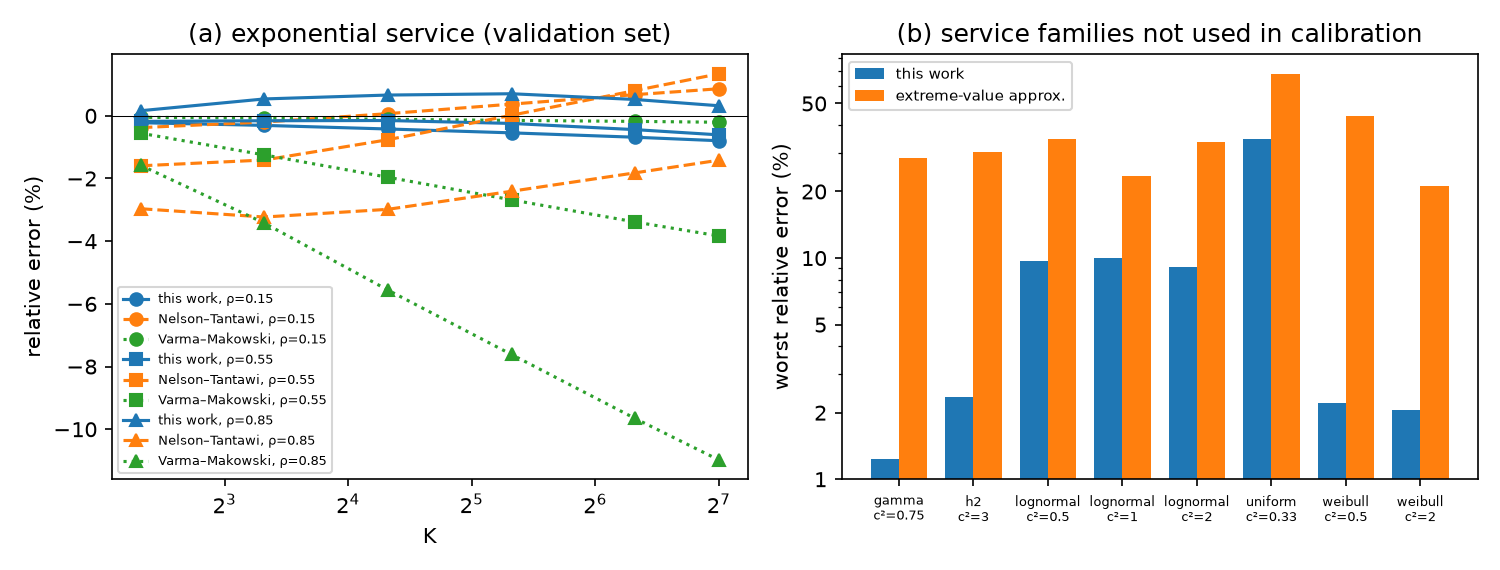
\includegraphics[width=\textwidth]{fig_errors.png}
\caption{(a) Signed relative error for exponential service as a function of $K$, for three loads. (b) Worst-case
error per service family never used in calibration (log scale).}
\label{fig:err}
\end{figure}

\section{Why it fails for uniform and lognormal service}

Correlation among servers arises only through the waiting times, which share the arrival process. The service times
themselves are independent. The factor $\phi$ in Eq.~(\ref{eq:main}) scales the whole excess $R^{\max}_K-R$, and it is
therefore implicitly calibrated on how that excess splits between waiting and service.
\begin{itemize}
\item \textbf{Uniform service.} The service time is bounded, so for large $K$ the excess is dominated by the waiting
tail. That tail is strongly correlated across servers, so $\phi$ is overestimated.
\item \textbf{Lognormal service.} The excess carries a larger independent, service-driven share, so $\phi$ is
underestimated.
\end{itemize}
After the confirmation we explored two refinements, using the confirmation data as new development data and holding
out one family at a time. Neither met the $5\%$ target.
\begin{itemize}
\item Applying the factor only to the waiting part left the uniform error at $26$--$28\%$.
\item A Gaussian copula on the waiting times, with independent service and correlation $r^{1.4}$, reduced it to
$12$--$16\%$, but left lognormal at about $12\%$.
\end{itemize}
A shape-aware model of the dependence, beyond $(\rho,c^2,K)$, appears necessary.

\section{Conclusions}

Eq.~(\ref{eq:main}) is a five-constant correction of the classical independence bound. On a preregistered test it is
about three times more accurate than Nelson--Tantawi for exponential service up to $K=128$, and within $2.4\%$ for
unseen gamma, hyperexponential and Weibull service. It is not reliable for bounded or lognormal service. The exact
ingredients ($R$ and $R^{\max}_K$) are inexpensive to compute for any service distribution. A reference
implementation and all data are available as ancillary files.

\paragraph{Acknowledgments.} Large parts of the code and text were drafted with the assistance of an AI system (Claude,
Anthropic). All results were produced by the preregistered scripts and checked by the author.

\begin{thebibliography}{99}
\bibitem{FlattoHahn1984} L.~Flatto and S.~Hahn, Two parallel queues created by arrivals with two demands I,
\emph{SIAM J. Appl. Math.} 44 (1984) 1041--1053.
\bibitem{NelsonTantawi1988} R.~Nelson and A.~N.~Tantawi, Approximate analysis of fork/join synchronization in
parallel queues, \emph{IEEE Trans. Computers} 37 (1988) 739--743.
\bibitem{VarmaMakowski1994} S.~Varma and A.~M.~Makowski, Interpolation approximations for symmetric fork-join queues,
\emph{Perform. Eval.} 20 (1994) 245--265.
\bibitem{ThomasianTantawi1994} A.~Thomasian and A.~N.~Tantawi, Approximate solutions for M/G/1 fork/join
synchronization, \emph{Proc. Winter Simulation Conference} (1994) 361--368.
\bibitem{Thomasian2014} A.~Thomasian, Analysis of fork/join and related queueing systems, \emph{ACM Comput. Surv.}
47(2) (2014) 17.
\bibitem{ThomasianRAID} A.~Thomasian, RAID organizations for improved reliability and performance: a not entirely
unbiased tutorial, arXiv:2401.03235.
\bibitem{Baccelli1989} F.~Baccelli, A.~M.~Makowski and A.~Shwartz, The fork-join queue and related systems with
synchronization constraints: stochastic ordering and computable bounds, \emph{Adv. Appl. Probab.} 21 (1989) 629--660.
\bibitem{Rizk2015} A.~Rizk, F.~Poloczek and F.~Ciucu, Computable bounds in fork-join queueing systems,
\emph{Proc. ACM SIGMETRICS} (2015) 335--346.
\bibitem{Liu2024kan} Z.~Liu et al., KAN: Kolmogorov--Arnold networks, arXiv:2404.19756.
\end{thebibliography}

\end{document}
